\chapter{Evaluation \& Discussion}

In this chapter, the focus will be on evaluating and discussing the project and, most importantly, two forms of DNS abuse, which are confusable domains and phishing due to their popularity among bad actors by testing and validating them.  The chapter will dive into real-life examples to illustrate the severity of these threats and examine existing mitigations and techniques used to mitigate them, to test how well the project met the objectives. In addition, a proposal will be made to improve the transparency around these mitigation strategies to foster accountability and trust. Through the analysis, the feasibility of implementing such transparency measures will be assessed by performing an analysis using data and evidence. Finally, the limitations of the work will be addressed. 


\section{Confusable Domains}
\subsection{Identification \& Examples of Targeted Domains}

The choice of such domains to target and outsource depends on many factors, each with its implications on business strategy, marketing, and law enforcement. The selection of these domains hence matters a lot in creating potential conflict, especially those related to existing trademarks. Understanding these selection criteria is very important in trying to negotiate the hurdles of the digital market and in protecting rights through intellectual property.

\begin{itemize}
  \item \textbf{Commercial Appeal:} The domains with commercial appeal attract traffic and can generate income. They are short and memorable and relate to popular products or services, sometimes leading to ownership arguments \cite{Li2002ConflictDomainTrademark}.
  
  \item \textbf{Keyword Relevance:} Similarly, a domain specific to keywords ranks well in the search and indirectly lures organic traffic, which will help enormously the business in the search for common search queries and, in this process, generates more clicks.
  
  \item \textbf{Similarity to Well-known Trademarks:} Domain names, when similar to those of famous trademarks, can cause legal trouble for the trademark owner. laws prevent confusion and protect the brand reputation in disputes.
\end{itemize}

\subsection{Real-life examples}

\begin{itemize}
    \item \textbf{Cybersquatting :} A famous case was of Amul in 2019-2020. The renowned dairy giant had an impersonation case of similar domain registration, which was used to lead the public toward phishing, such as for fake distributorship or job opportunities. The Indian dairy brand above had this issue repeated three times in the last three years, namely from 2018 to 2020, and the company had to publish public notice while sending legal bodies, which also exhibited to readers the extent to which one can go for the brand defence issue.\cite{MehtaCybersquatting}.
    
    \item \textbf{Typosquatting :} One of the US healthcare providers, Elara Caring, gives an illustrative example of a cyberattack it encountered in December 2020: as a result, the following breaches in healthcare cybersecurity were defined: unauthorised access to email accounts of staff members. The breach, which lasted for a week, underscores the need for an improved incident response \cite{PandaSecurityPhishing}.
    
     \item \textbf{Reverse Domain Name Hijacking  :} is the act of trademark owners trying to take a domain away from its rightful holder based on the claim of trademark rights, considering that he holds a bona fide registration over the said domain. It may also be described as the use of legal or dispute resolution mechanisms to try to force people from their domains \cite{Sun2006DomainTrademarkConflict}.  An RDNH was claimed in a UDRP action against "groovle.com," in which the domain was purported to be too close to Google's trademark. However, since the domain was used for another search engine, it was deemed legitimately used and did not violate Google's trademark or be registered in bad faith \cite{Singh2011ReverseDomainHijacking}.
\end{itemize}


\subsection {Homograph attacks} 


The risk of continued homograph attacks is in using characters that look similar and thus mimic trusted domain names, such as using a lowercase "l" (el) to look like an uppercase "I" (eye) in the name "paypal.com" vs. "paypaI.com". The introduction of International Domain Names has only expanded the scope of such attacks, yet their prevalence is less. Still, the growing trend of more and more phishing attacks and how easy it is to fool users by taking them to fake sites require eternal vigilance. As a result of a new study, "Cutting through the confusion" \cite{holgers2006homograph}, it is going to reveal the scale and potential threat to homograph attacks, such as visual similarity between characters from different scripts, like Cyrillic or Greek, which is displayed in punycode in browsers, when attackers register domains that are visually similar to legitimate ones. This can be summarised in the table below, showing possible and actual registrations of such deceptive domains; hence, bringing out the difference between potential and actual use of the deceptive domain. For example, the domain "yahoo.com" had more than 5000 potential homograph variants, with only two actually registered, and "google.com" had a thousand possibilities, with four actual registrations.This is indicative of the importance of developing early preventive development and raising awareness of the risk from homograph attacks, as it sets into a very necessary chain of understanding mechanics and scope of homographs prevalence. Figure \ref{fig:figureAlot1} clearly shows, by means of a graphic illustration, the scope and scale of homograph attacks, which point to the potential risks that these attacks could pose to online security and the awareness and mitigation strategies that need to be implemented to protect Internet users from such deceptive practices. 

\captionsetup{font= footnotesize}
\begin{figure}[H]
    \centering
    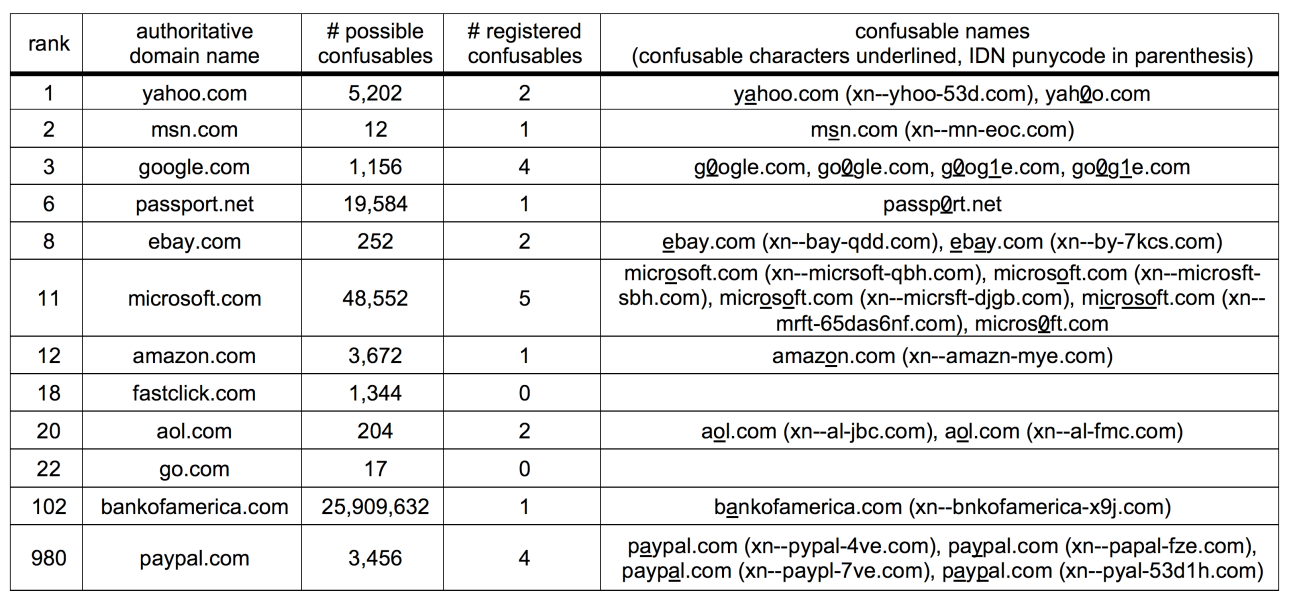
\includegraphics[width=1\linewidth]{evaluation/confusable.png}
    
    \caption{confusables registered for popular domains, adapted from \cite{HomographAttacks}.}
    \label{fig:figureAlot1}
\end{figure}

\subsection{ Real-life Mitigations}

The following scenarios are examples of real-life confusable domain mitigations :

\begin{itemize}
    \item \textbf{Cloudflare's Zero Trust Services Approach :} The Cloudflare Zero Trust Services stops the domain used to mimic the real domain by equipping businesses with anti-phishing protection through Cloudflare Gateway. This protects corporate networks from phishing, using the trust element of well-known brands \cite{Cloudflare2023}. This is initiated in the system when making the very first query to any domain through a DNS resolver of 1.1.1.1, which in turn initiates a fuzzy matching protocol for analysis and comparison with a database of potential phishing domains. This should issue alerts on domains that are similar to those of legitimate brands, hence easily detecting them promptly and for quick response. Cloudflare enables monitoring 24/7 in real time with historical analysis, offering security teams the alert of domain matching certain patterns, hence being suspected, for fast review and action if the domain has shown up within 30 days. Cloudflare further supports with criteria to specify the corresponding investigation in .json, based on given domains or patterns, and may be subject to security risks.

     \item \textbf{IDN Handling of Google Chrome : }Google Chrome enforces an IDN (Internationalised Domain Names) policy to determine in which unicode or punycode form a domain label should be displayed. The domain label is tested to determine whether it has mixed script, invisible characters, or visually confusable characters, and whether it is actually validly converted to Unicode. For instance, domains containing characters of different scripts, or those that are clearly identified as mixed script confusables, will be displayed in punycode, warning the users of potential deceptions. Chrome also offers comprehensive warnings for secure URLs that appear to be an imitation of already known Web pages \cite{ChromiumIDN}.
     
\end{itemize}

\subsection{Techniques for Mitigating Confusable Domains}

Mitigating confusable domains requires sophisticated techniques tailored to address the unique challenges presented by both non-Internationalised Domain Names (non-IDNs) and Internationalised Domain Names (IDNs). The threat of these two groups is vastly different and the technical possibility of most mitigation strategies also varies greatly. The subsequent section of the paper describes the mitigation methods in detail, addressing their operational feasibility and potential collaboration initiatives.

Non-IDNs Mitigation Techniques: These techniques aim to detect and mitigate domain squatting and typosquatting, where the attacker registers a typographical error or variant of a legitimate domain so that users get confused.

\begin{enumerate}
  \item Registry-Level Measures: Domain registries can implement checks to prevent the registration of domains similar to existing trademarks or brand names, using algorithms to detect variations and misspellings closely similar to protected names \cite{WTR2020}.
  \item Trademark Protection Programmes: Trademark Clearinghouse (TMCH) offers mechanisms for trademark owners to protect their rights by receiving notifications when someone attempts to register a domain that matches their trademark \cite{ICANNTMCH}.
  \item Automated Monitoring and Reporting: Automated systems can continuously monitor domain registrations for names that closely resemble known trademarks or brand names, allowing rapid detection and legal action against infringers \cite{TMCH2023}.
\end{enumerate}

IDNs Mitigation Techniques: The problem with IDNs is the potential for homograph attacks, where attackers can use characters from different scripts that visually appear to look like characters in Latin script.

\begin{enumerate}
  \item Punycode Awareness and Monitoring: Web browsers and security tools convert IDNs to punycode, a representation that encodes Unicode characters in ASCII. Awareness of punycode and monitoring for suspicious registrations can help identify potential homograph domains \cite{SOCRadar2023}.
  \item Browser-Level Defences: Modern web browsers have implemented defences against IDN homograph attacks by displaying the punycode version of the domain or alerting users when a domain name contains characters from multiple scripts \cite{Malwarebytes2017}.
  \item Collaborative Blacklisting and Sharing of Threat Intelligence: Organisations can collaborate to share information on known malicious IDNs, contributing to comprehensive blacklists that can be used by registrars, DNS providers, and end users to block access to malicious sites \cite{CyberThreatAlliance2023}.
  
\end{enumerate}


\subsection{ Transparency in Mitigation Efforts}

The element of transparency in dealing with confusable domains will be a great support in protecting the Internet from malicious activities such as phishing and trademark infringements. This encompasses a set of practices by domain registries and registrars to identify and publicise those domains that could mislead due to their similarity to legitimate ones. It contains means of transparency, such as publishing lists of those domains to alert the community about possible threats and taking secure measures, if possible.

\begin{itemize}
  \item \textbf{Cloudflare's Zero Trust Services Approach: }Cloudflare's process for identifying and blocking confusable domains should be transparent to its users. This includes detailing the criteria for flagging domains as phishing sites and the mechanisms in place for users to appeal or request a review of blocked domains. By openly sharing the methodology behind their zero-trust rules and how they are applied through the Cloudflare Gateway, trust in Cloudflare's protective measures is bolstered among corporate networks.
  
  
  \item \textbf{IDN Handling of Google Chrome:} Transparency from the side of Google Chrome for the display of domain names helps the user understand the risks to their security. How policy could be properly executed, reported, or suggested for changes by the community of users to increase internet safety will also be explained.

  \item \textbf{Typo-squatting Detection Tools: }The similar methodology should be evident in how similar domain names are detected by tools such as DNStwist or URLCrazy and how it could be detected and shared in a proactive security setup, which could also help others in any organisation.
  
  \item \textbf{Collaborative Efforts and Intelligence Sharing: }The partnership between cybersecurity entities and domain registrars, as well as initiatives such as the Anti-Phishing Working Group (APWG), should prioritise transparency in their operations. This includes the sharing of methodologies for threat detection, the criteria for taking action against malicious domains, and the processes for stakeholders to contribute or access shared intelligence. Transparency in these collaborative efforts ensures that actions taken against confusable domains are fair, understood by all parties involved, and supported by a broad community of internet security stakeholders.
  
 \item \textbf{Transparency for non-IDN registries : } 

 \begin{enumerate}
  \item Registry-Level Measures: Transparency in level-registry measures becomes a necessity if trust has to be kept between registrants and domain trademark owners. They are published criteria and algorithms used to find variations and misspellings of names submitted for protection. Making these publicly available can then ensure fairness, and feedback in detecting mechanisms is therefore paved for improving them.
  \item Trademark Protection Programmes: Communication is openly clear about all operations; this includes verification and notification. The guidelines make it easier to understand the rights and measures to protect your brand.
  \item Automated Monitoring and Reporting: set by the criteria and thresholds for informing the brand owners about the protection level for their trademark, and thereby will enable improved monitoring.
  
\end{enumerate}
 
 \item \textbf{Transparency for IDN registries  : } 

  \begin{enumerate}
  \item Monitoring and Identifying Measures for Suspicious Punycode Registrations: All domain registrars and trademark owners, together with security professionals, must adhere to measures on suspicious punycode registrations. Publicising the details of activities carried out to monitor them propagates homographic threats through collective ideas, also in their identification and mitigation.
  
  \item Browser-Level Defences: Web browsers have an important role in the defence of homograph attacks. They have to explain clearly to the user their defence mechanisms, such as ways of displaying punycode domains and ways of raising warnings so that they can be understood and trusted.
  
  \item Collaborative Blacklisting and Shared Threat Intelligence: Threat intelligence should be collaborative, based on a set of criteria, to blacklist domains. Clear rules on how to submit, validate, and remove data can also enhance the fairness and trust in collaborative security efforts.
\end{enumerate}
  
  
\end{itemize}

In summary, transparency in all these mitigation techniques not only builds trust between users, developers, and organisations, but also enhances the collective ability to respond to and prevent threats posed by confusable domains.


\subsection{ Analysis : Feasibility \& Practical Challenges}

 \begin{enumerate}
  \item Automated Monitoring and Reporting: Feasible; Technology exists to automate monitoring, even though the refinement of algorithms to decrease false positives and negatives from human review can probably not be undertaken with existing resources.
  \item  Punycode Registration Monitoring: Feasible; It will mainly require the use of existing technology and cooperation that could be initiated with little difficulty between stakeholders.
   \item Cloudflare's Zero Trust Services Approach: Feasible; since well-architected infrastructure and broad adoption have made Cloudflare zero-trust rules simple and effective to deploy, with a balance of security and operational efficiency without seismic root and branch changes.
  \item IDN Handling of Google Chrome and Browser-Level Defences: Feasible; Given that Chrome today has an enormous user base and that the groundwork for stopping homograph attacks already exists, it stands to reason that a solution is reasonably possible, meaning not too difficult, within a set timeline, and within the lifespan of any other typical software product.
  \item Blacklisting and Threat Intelligence Sharing: Moderately Feasible; Since agreement could be reached on shared platforms and protocols, but they imply strong cooperation and trust among such diverse entities, which is unlikely to be developed fast.
  \item Trademark Protection Programmes: Moderately Feasible; They are well-functioning processes under such adequate structures like TMCH and can be learnt while proceeding with experience, but likely to face legal and operational issues.
  \item  Browser-Level Defences: Not Feasible; While this is technically feasible, it seems rather infeasible soon that user practices will become uniform across all web browsers and that all users will be well trained in various security practices.
  \item Registry-Level Measures: Not Feasible; this would require very heavy coordination and agreement on standards across diverse jurisdictions and registries.
 

  
\end{enumerate}

\section{Phishing}

\subsection{Real-life examples}

\begin{enumerate}
    \item InterMed and Spectrum Healthcare Partners fell for a major phishing attack on 44,000 patient data. The InterMed breach involved clinical information for 33,000 patients, specifically names, birthdates, insurance, and some social security numbers, from 4 to 10 September. In another case, Central Maine Orthopaedics is reported to have breached 11,308 of their patient record files by unauthorised access to emails that contain personal and clinical details. It is such an incident that really makes it very paramount to strengthen email security and at the same time to provide professional training on data protection \cite{HIPAAJournal2020Phishing} .
    \item Google and Facebook were almost fooled by a group of phishers into a \$100 million sophisticated scam in which they were imitating legitimate invoices from the suppliers. The case is one among many that have caused the vulnerability of technology firms to social engineering and the need for reinforced security, employee training, and verification processes to combat ever-changing cyber threats \cite{CNBC2019Phishing}.
\end{enumerate}

\subsection{Real-life Mitigations} 

\begin{itemize}
    
     \item \textbf{Comprehensive Security Measures :} LaptopMD points out that the risk of ignorant searches requires the formulation of policies that make it difficult to land on some sites. In addition to this, the awareness of phisher techniques and browsing issues by employees will greatly save them from being caught in cases of phishing \cite{DigitalGuardianPhishingPrevention}.
     
     \item \textbf{Technological \& Human Factors :} Combining technology with awareness, SecureHIM advises that both should be combined by any organisation to include spam filters and two-factor authentications with the vigilance of employees to detect and eliminate the risks of phishing \cite{DigitalGuardianPhishingPrevention}.
     
     \item \textbf{Awareness against unsolicited emails :} The Centre for Democracy and Technology outlines the training that should be provided to avoid activities such as phishing, including the need not to respond to unsolicited emails even when suspecting anything fishy \cite{CDTPhishingMitigation}.
     
     
\end{itemize}

\subsection{Techniques for Mitigating Phishing}

Current phishing attack mitigation techniques focus mainly on preventing phishing
emails from reaching users' inboxes and discouraging users from accessing
phishing websites \cite{Suzuki2021Phishing}.

\begin{enumerate}
    \item Email filters: It uses algorithms that filter phishing emails, based on the reputation of the sender, the embedding of the link, and suspicious keywords, so that these emails cannot reach the inbox.
    \item Domain blocking: Take steps to block access from within an organisation's network to known phishing sites so that the organisation's users do not stumble on them accidentally.
    \item User Training: Train users on how to recognise signs from phishing emails and the risk associated with clicking on unknown links or sharing personal and sensitive information.
\end{enumerate}


The idea of a detailed thinking process of the offender, along with the description of the attributes in the environment that allow the attack to occur, is introduced with the Situational Crime Prevention Approach \cite{Suzuki2021Phishing}: This method was developed considering the theory that it is possible to deter potential attackers if the level of effort they make, the risk they take, and the likely rewards they receive are raised, stay the same, and lowered accordingly. It is worth mentioning that the criminal perspective is necessary to understand, and creating a hostile environment for phishing operations by implementing certain strategic preventive measures is crucial. This method includes the following steps:

 

\begin{enumerate}
    \item Increasing the Effort for Attackers: Implement strong authentication mechanisms and encryption to increase the difficulty of accessing or spoofing phishing websites or legitimate email accounts.
    \item Clarifying User Responsibilities: Information about users' role in security, such as awareness of phishing signs and reporting aids.
    \item Enhancing Detection Probability: Using the latest detection technologies and threat intelligence to recognise and eliminate phishing threats on time.
    \item Limiting Phishers' Access: Limiting the breadth of information that is accessible to the public, which might be used to construct compelling phishing emails and fake the identity of someone else or an organisation.
    \item Discouraging Future Attacks: Implement punitive actions such as tracking down familiar attackers and sharing information about the attack with a larger group of people to deter repeat offenders.
\end{enumerate}

This measure is designed not only to stop a phishing attack, but rather to create an environment that would lead to the cost-benefit ratio for phishing not so appealing to the attackers. Comprehensive perspectives on addressing phish through the three methods above singularly go to dramatically lower the vulnerability of organisations and individual persons to such acts.

In addition, Phishlimiter \cite{Chin2018PhishLimiter} , which is a new phishing detection and mitigation approach using Software-Defined Networking where it first proposes a new technique for deep packet inspection (DPI) and then leverages it with software-defined networking (SDN) to identify phishing activities through email and web-based communication. This is how it works:

\begin{enumerate}
    \item Deep Packet Inspection (DPI): Examines the network packet data more than the basic header information. Used to look at the content of packets looking for known signatures and patterns associated with phishing.
    \item Store and Forward (SF) and Forward and Inspect (FI) modes: SF mode temporarily stores packets for a thorough inspection before forwarding, while FI mode prioritises immediate forwarding with a parallel inspection to reduce latency.
    \item Artificial Neural Network (ANN): A machine learning model used to classify network traffic based on characteristics to detect links to potential phishing signatures.
    \item Dynamic adjustment of network flows: In the case of standard recognition, the system can dynamically change the routing to bypass the link or reduce flow to prevent the phishing process.
    \item Minimal disruption to network services: Designed to maintain the mitigation process minimised without targeting performance to ensure that final services would run smoothly even during the measure.
\end{enumerate}

\subsection{Transparency in Mitigation Efforts}

Here is how transparency can be applied to each of the mitigation techniques described:
\begin{itemize}
    \item \textbf{Employee Awareness and Training :} 
    
    Communication: This will consist of clearly informing the employees about the kind of threat and what it could mean for the organisation and their role in these defences.
    
    Accessibility: Make people aware that the repository exists, or make the resources easily available for reference. 

     \item \textbf{Comprehensive Security Measures: }
     
     Policy Publishing: All available policies, especially those related to web browsing, email attachments, and the use of security tools, will be published openly to let employees know about them.
     

    Changes and Updates: Introduce the workforce to changes relating to security measures and how such changes are beneficial and serve as a cover against new hazards.

     \item \textbf{Technological \& Human Factors: } 
     
     Tool Transparency: Clearly state the tool and the reason for its being in place for security (e.g., spam filters, two-factor authentication), and its work on subduing phishing. 
     
    User Control and Visibility: Attempt to give users some form of control or visibility over the security tools through which their work could be affected. Feedback from a blocked phishing attempt could, for example, help to reinforce the training.

     \item \textbf{Awareness against unsolicited emails:  } 
     
     Open Communication on Threats: Constant updates on new phishing techniques and any other notable attacks are discussed among the industry to be updated.
     
    Best practices: Develop best practices for easy identification and to be visible on how to catch and react to phishing attacks, with graphic examples or checklists.

    \item \textbf{Email Filters:} 

    The effectiveness of email filtering technology in mitigating phishing attempts is enhanced by transparency in its operational parameters. This helps to make the user understand, starting from analysing the reputation of the sender to the various steps related to decision making of phishing keywords. Continuous improvement builds trust, and perhaps some community members might even wish to provide feedback on how to improve the performance of the filters or report inaccuracies to the filter system regarding combat against the threats of phishing.

    \item \textbf{Domain Blocking:} 

    Such measures may include transparency in the criteria of the blacklisting and regular updates in relation to the access to the known phishing sites inside the organisation's network. This implies also setting a clear means of reporting unlisted phishing sites and correcting false positives by stakeholders. 

    \item \textbf{Situational Crime Prevention Approach (SCP):}

    The major advantage of the SCP approach is the clear disclosure of both the applied methodology and the results obtained. This is through the explanation of the analysis of the criminal's thought and environmental factors aiding phishing, whereby the stakeholders are enlightened, therefore, they make efforts to reduce it. 

    \item \textbf{Phishlimiter:}

    The phishing detection system, such as the DPI integrated with SDN, has the ability to make its operation transparent, may increase user confidence, and preserve system functionality. It could emphasise the reliability and credibility of such a system if the criteria and algorithms by which the system determines a potential phishing attack are clearly spelt out. 

\end{itemize}

\subsection{ Analysis : Feasibility \& Practical Challenges }

\begin{enumerate}
    
    \item Comprehensive Security Measures :Feasible; The deployment of web filters and secure browsing policies is technically straightforward with existing technology. The main effort lies in the continuous update of policies and employee education.
    \item Technological and Human Factors: Feasible; The integration of spam filters, two-factor authentication, and secure browsing add-ons is readily achievable with current technology. The human element, continuous employee vigilance, enhances the effectiveness of these tools without significant additional costs.
    \item Awareness against unsolicited emails: Feasible; Establishing and communicating best practices for handling suspicious emails involves minimal costs and leverages existing communication channels within organisations.

     \item User Training: Feasible; The training of the user's awareness on phishing is practical and beneficial, as it allows giving room for the user to measure the feedback on the effectiveness of training and to give suggestions for improvements that can enhance programme accessibility and user participation.
     
     \item Situational Crime Prevention Approach (SCP): Feasible; sharing information that identifies how an offender behaves and the environment that helps him/her attack. Although presenting this success story is of great value, great care must be taken in the handling of the detailed analyses of criminal tactics to avoid misuse. Community feedback will allow for further development.
     
     \item Domain Blocking: Moderately Feasible; Updating blacklists and dealing with the false positives, which have to be dealt with. This is a mammoth task, especially for relatively smaller organisations with few resources at their disposal. The process demands balance in responding very accurately within a very short time, which can over-stretch resources.
     
    \item Email Filters: Not Feasible;  Describing the general criteria and algorithms for email filtering is possible, but full disclosure risks security by enabling attackers to circumvent these measures. Partial transparency can be achieved without compromising the integrity of the system.
    
    \item Phishlimiter: Not Feasible; The complexity and proprietary nature of technologies like DPI and SDN make full disclosure of Phishlimiter's operations impractical. Detailed investigation of operations could compromise security. Keeping up with evolving phishing tactics requires continuous updates, which may not always be promptly disclosed to avoid aiding adversaries.
    
\end{enumerate}


\section{Collaboration Among Registrars, Registries, and DNS Collaborators}

This collaboration should be achieved with the DNS registry, the registry, and the collaborators. In that way, they can boost common resources and intelligence that can guide making the Internet more secure and resilient. This strictly falls within the remit of registries and registrars acting in collaboration to put in place such stringent registration policy with procedures for verification, checking against mimicking existing trademarks or even popular domain names. In this way, the collaboration can even manifest itself through the sharing of sensitive data with regard to domain abuse threats and trends. Databases and threat intelligence platforms are shared amongst stakeholders, allowing them to anticipate and avert most such perils well before they impact netizens. This collective effort will enable the formulation of standards by which to coordinate responses to confusable domain incident reports. Mitigating confusable domains and phishing requires that registrars, registries, and DNS collaborators work together in a common effort. This is due to the increasing level of threats and the shared responsibility of all actors involved in the DNS ecosystem \cite{Catania2022}. To put this into perspective, here are some examples: 


\begin{enumerate}
  \item New specifications on defining DNS abuse have been entered into ICANN’s contracts from ICANN’s contracted parties. Furthermore, there are clear requirements that define the actions to be taken by registry and registry after receiving immediate actionable evidence of abuse. This move clarifies the roles that different stakeholders can play in addressing the DNS abuse issue and establishing a common approach to redress \cite{Weinstein2023}.
  \item Some of these new duties have been positively approved by the community. The community supported the new obligations of the ICANN contract parties to further mitigate DNS abuse. The message that this example sends to everyone is that the community is willing to join and participate in DNS abuse and other challenges to address \cite{ICANN2023}.
  \item  Efforts such as NetBeacon, with the support of the DNS Abuse Institute, are being rolled out to reduce friction in reporting and mitigating DNS abuse. This service solves the current complexities and quality standards associated with the reporting of DNS abuse, as it makes the work easier for registrars, ultimately narrowing down their scope to the relevant and evidenced report, and underlines the need for cooperation among registrars, registries, and other DNS stakeholders. This is what is capable of saving the Internet and, at the same time, protecting the credibility and confidence of DNS \cite{NetBeacon}.
  
\end{enumerate}

Real-life examples of entities seeking to block the resolution of DNS names used by bad actors for phishing and other malicious activities, especially in connection with public recursive DNS servers, frequently revolve around matters of control, filtering, or securing internet traffic with various kinds of motivation corresponding to such sectors. Consider the following:

\begin{enumerate}
    \item Governmental Efforts to Block DNS Resolutions: Governments may interfere directly with DNS operations to enforce some censorship or block access to particular types of content. For instance, China uses the Great Firewall for regulation of access to the World Wide Web within their territory, including doing some DNS mismanagement to block unwanted content \cite{XuAlbert2017MediaCensorship}.
    \item Corporate and ISP DNS Filtering: DNS filtering can be deployed by companies and even ISPs in a bid to achieve enhanced online security. For instance, Heimdal Security explicates how DNS filtering works as one of the measures to prevent their access to various harmful or inappropriate websites since it first checks the requests for domains. If some areflagged, access is denied, hence maintaining both security and productivity within one's organisation. This approach is very effective for the prevention of phishing and malware attacks because it stops DNS requests towards malicious sites \cite{
HeimdalDNSSecurity2023}.
    \item Ad Block DNS Services : Cloudflare discusses how DNS filtering can be used to prevent access to malicious sites and also filter what is harmful or unfit for viewing. This is done at the DNS level to prevent these sites from loading on devices. Cloudflare uses its DNS to filter part of a more prominent access control policy, which is an effort to secure company data and govern what employees will see on the network they manage \cite{CloudflareDNSFiltering2023}.   
\end{enumerate}

 On the negative side, attackers are taking advantage of DNS blocking mechanisms to carry out DNS-based attacks. These include using DGAs (Domain Generation Algorithms) for malware communication, using FastFlux techniques for slip-streaming attacks, basically creating malicious newly registered domains (NRDs) that appear benign and legitimate to an outside observer, etc. All this makes it difficult to block bad content at the DNS level, which calls for quite sophisticated countermeasures.


\section{Benefits of Transparency }


Transparency has numerous advantages when it comes to handling confusable domains and mitigating phishing. First, it encourages domain registry owners and registrars to be more accountable to each other by motivating them to take an active role in the identification and removal of confusable domains and phishing websites. Second, openness discourages bad actors who might otherwise take advantage of the anonymity provided by a lack of public monitoring. Third, by making these lists available to the public, registries and registrars enable companies and trademark owners to promptly take precautionary measures to safeguard their brands, including acquiring domain names or pursuing legal action. Transparency also facilitates community-based mitigation initiatives, in which researchers studying cybersecurity and the broader community work together to detect and eliminate dangers. This coordinated effort not only tackles confusable domains, but also considerably impedes phishing attempts by revealing, and thus reducing, the strategies employed by bad actors. The effectiveness of these tactics is significantly increased by using the collective expertise and attention to detail of the cybersecurity community, resulting in a more secure online environment for all parties involved.


\section{Drawbacks and Security Concerns} 

At the same time, the issue of publishing confusable domain lists, while ultimately beneficial for cybersecurity, also implies several limitations and security issues, such as the problem of phishing. First, the reason for concern is that publishing these lists can serve as a manual for bad actors since it potentially discloses potential domains for phishing. For example, if victims are exposed in such a way, bad actors can quickly adjust their approaches, ensuring that their activities stay one step ahead of countermeasures. Second, false positives, or legitimate domains that are mistakenly identified as confusable, also represent a serious challenge. For real businesses and people, a loophole for that is their potential association with phishing since this can entail unnecessary attention, legal action, and reputation damage. Third, the issue of transparency also raises concern about how relevant releasing such data is in terms of attack prevention. While the logic of making the lists available to the public before they can be misused for abuse, such as phishing, is clear, the sheer volume of domain registration and the continuous changes in domain abuse tactics undermine their actual usefulness for end-users and organisations to proactively identify and tackle phishing risks.



\section{Limitations of Research Conducted on DNS Abuse Transparency }

\begin{enumerate}
    \item Variability in reporting standards: The majority of challenges faced in actual practice come with a lack of uniformity in standards from DNS infrastructure providers from the definition of abuse to the thresholds of actions and how those actions are being reported. This inconsistency has made efforts to collect and compare the data of different entities difficult to piece together into one coherent picture for sensible enforcement of DNS abuse mitigation. 

    \item Limited Availability of Data: The general lack of transparency reports that are available to the public. Providers either do not at all release or do, and in doing so, have an omission of information required to be looked into. This means that there are still gaps in understanding the whole spectrum of strategies deployed by the DNS abuse domain due to data unavailability. 
    
    \item Reluctance to Share Sensitive Information: Information provided by respondents about abuses and what they do to mitigate them. In general, concerns about privacy, security, and the potential of revealing vulnerabilities to bad actors contribute to this reluctance, which leads to Limiting the capacity of researchers to perform a comprehensive analysis of DNS abuse mitigation strategies.
    
    \item Dynamic Nature of DNS Abuse: The evolving tactics employed by those who abuse DNS are constantly changing, so results can be out of date very fast. It is more difficult to create best practices that are applicable and efficient over time due to this quick change. Because DNS abuse is dynamic, it requires ongoing research and strategy adaptation to stay ahead of new threats.

    \item Potential Bias in Self-Reported Data: Self-reporting in transparency reports can still bias the results. Organisations tend to emphasise their achievements while downplaying their shortcomings or difficulties. Due to this biased reporting, opinions about how well DNS abuse is being controlled can be distorted, which could cause mitigation efforts to be overestimated.
    
    \item Complexity of Measuring Impact: Due to the specific nature of the Internet ecosystem, it is quite challenging to evaluate the efficacy of DNS abuse mitigation techniques. Furthermore, the evaluation process is quite complex due to the indirect impact of specific actions of DNS abuse prevention efforts on the larger effects.

    \item International and Jurisdictional Challenges: Due to the international scope of the Internet, different legal and regulatory frameworks in different jurisdictions have an impact on DNS abuse and how it is mitigated. These differences highlight the need for cross-border cooperation and harmonisation by adding complications to the implementation and evaluation of transparent practices on an international scale.

    \item Ethical and Privacy Considerations: Ethical issues related to data collection and analysis that may include sensitive or personally identifiable information must be addressed in research in this field. Respecting ethical and privacy standards is very important, but it can also restrict the available research approaches, further limiting the breadth and depth of the study.
    
  
\end{enumerate}

As demonstrated, all these limitations show the complex difficulties in conducting a thorough research on DNS abuse mitigation transparency. Only by operating with the principles of team interaction, originality, and a willingness to develop research tools and approaches in the given area, can the misrepresentation difficulties be resolved.

\section{How well did the project meet the objectives?}

In evaluating the success and impact of the research project on DNS Abuse Transparency, a key question in assessing the achievements and influence of the study on DNS Abuse Transparency is addressed. To what extent did the project fulfil its original objectives? This section seeks to systematically evaluate the project's accomplishments in relation to its objectives, taking into account the intricate domain of DNS abuse and the difficulties associated with improving transparency and management procedures. A thorough review is provided by looking at stakeholder participation, the contribution to understanding DNS abuse, the objective achievement, and the practical consequences of the results. Shortcomings are acknowledged and recommendations for further research and development are made, recognising both the successes and the areas that still require improvement. This reflection not only demonstrates the progress gained but also the continuous path toward a DNS ecosystem that is more open, safe, and resistant to abuse.


\subsection{Objective Fulfilment}

The objective of these projects was to increase the understanding and transparency of stakeholders about reporting DNS abuse. Despite many challenges that the project faced, such as working with different reporting standards or limited access to data, this effort managed to uncover light flaws in the approach to mitigating and reporting DNS abuse. This project also demonstrated the high level of complexity and variety of approaches taken by different institutions in reporting, which accentuated the importance of unified and mandatory reporting requirements.

\subsection{Impact on Understanding DNS Abuse}

Given the difficulties, the research project yielded valuable information on the state of mitigation of DNS abuse. It showed that DNS abuse is unpredictable and, due to rapidly changing tactics of bad actors, mitigation measures should also be updated regularly. The study revealed several gaps in current knowledge and approaches to address, as shown by the lack of transparency reports and the unwillingness of providers to share critical data on their scopes. These findings could lay the ground for further research and policy-making.

\subsection{Stakeholder Engagement}

It was important to include interaction with stakeholders, including registry owners, policy makers, and DNS registry. The project encouraged discussion of the need for increased sector and jurisdiction cooperation and transparency. However, it seems that there is more to be desired in the impact on stakeholder behaviours and policies: for example, more proactive efforts and collaboration in the fight against DNS abuse.

\subsection{Practical Implications}
The outcomes of the project lead to positive results in the impact of transparency in reducing DNS abuse. Implementing recommendations for setting up standardised report creation processes and facilitation of data exchange could lead to more coherent and effective DNS abuse mitigation efforts. These recommendations provide practical next steps for stakeholders to better address the issues raised.

\subsection{Suggestions for Improvement}


Future projects, therefore, can discuss study questions on newly developed strategies, which abuse DNS, and research more aspects of transparency, so that they can obtain deeper insights. Further improvements in how to engage stakeholders include more transparency in forums to work with them toward the establishment of joint research projects, thereby increasing the scope and quality of information. Furthermore, promoting the idea of the project could lead to more noticeable changes in practice and policy.


\subsection{Future Vision}

This research project embarked on an extensive effort to clarify the complexity of the transparency of DNS abuse. Taking into account obstacles such as the dynamic nature of abuse methods and the availability of data, the effort achieved significant achievements in highlighting important areas for development and setting the stage for future breakthroughs. This development would represent a significant step forward in creating greater transparency and consistency in efforts to mitigate DNS abuse in recognition of the work being done and research and cooperation that will continue. Consequently, the way forward demands that all actors work together toward the recommendations for having a more secure, safe online environment.
